\begin{figure}[!t]
\centering
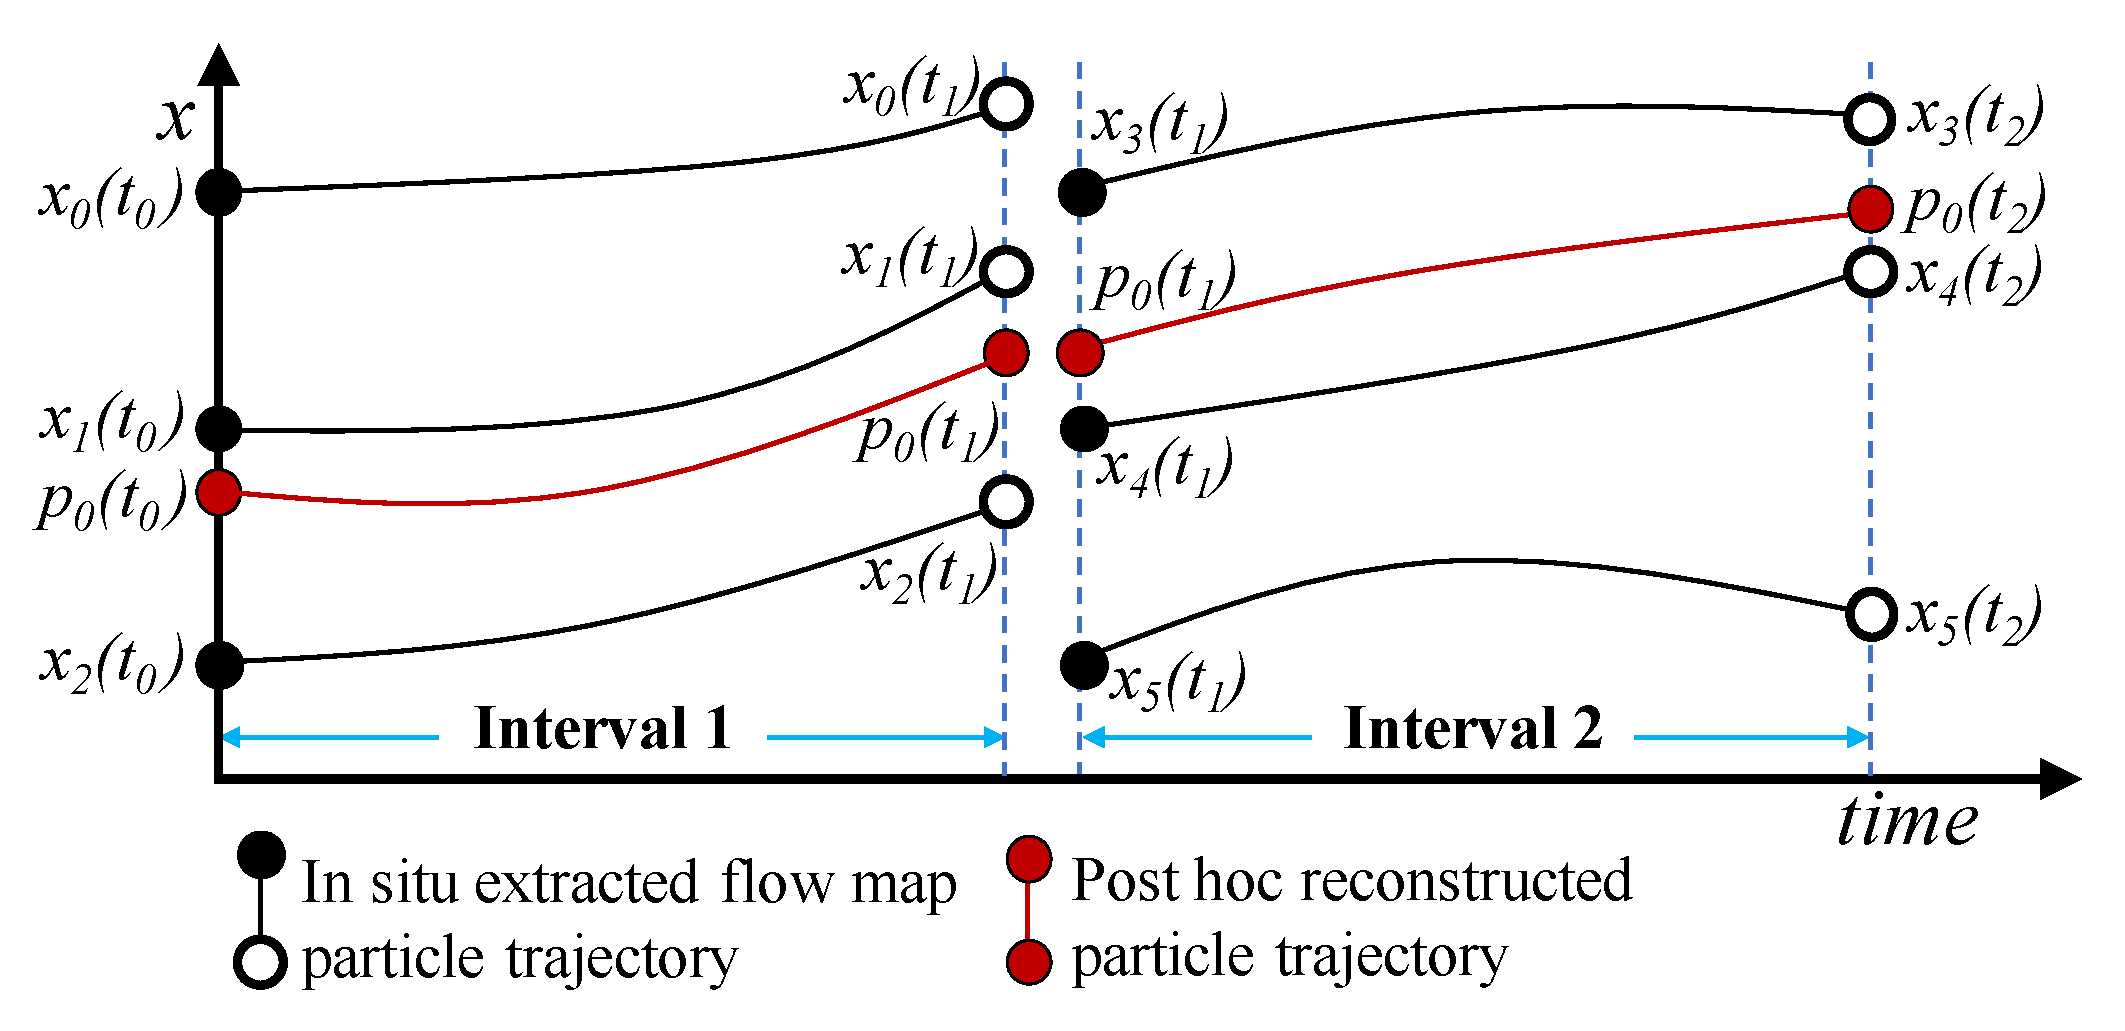
\includegraphics[width=\linewidth]{Images/phases_new_tall.pdf}
\caption{\fix{The phases of Lagrangian analysis. The in situ phase uses uniform seed placement and extracts flow maps over temporally nonoverlapping intervals. The extracted flow maps are used as input during the post hoc phase. In this example, the red particle's trajectory is calculated by interpolating the flow maps over two intervals of time.}}
\vspace{-6mm}
\label{fig:phases}
\end{figure}
